\begin{frame}{Distribution of Track Parameters}
    \centering
    % \underline{Basic Plot Parameters}
    \begin{itemize}
        \item Number of Tracks
        \item Track Charge
        \item Track $\chi^2$
        \item Track nDoF [in Backup]
        \item Track In Station [in Backup]
        \item Track nLayers [in Backup]
        \item Track Propagation Error
    \end{itemize}
\end{frame}

\begin{frame}{Distribution of Number of Tracks}
    \begin{columns}
        \begin{column}{0.45\textwidth}
            \begin{itemize}
                \item Overall a higher number of tracks in 2024
                \item Partially can be due to much higher muon rate in 2024
                \item See this talk to see the difference in backgrounds
                      \href{https://indico.cern.ch/event/1350790/contributions/5686387/attachments/2836819/4957405/Introduction.pdf}{12
                          April General Meeting}
            \end{itemize}
        \end{column}
        \begin{column}{0.8\textwidth}
            \begin{figure}
                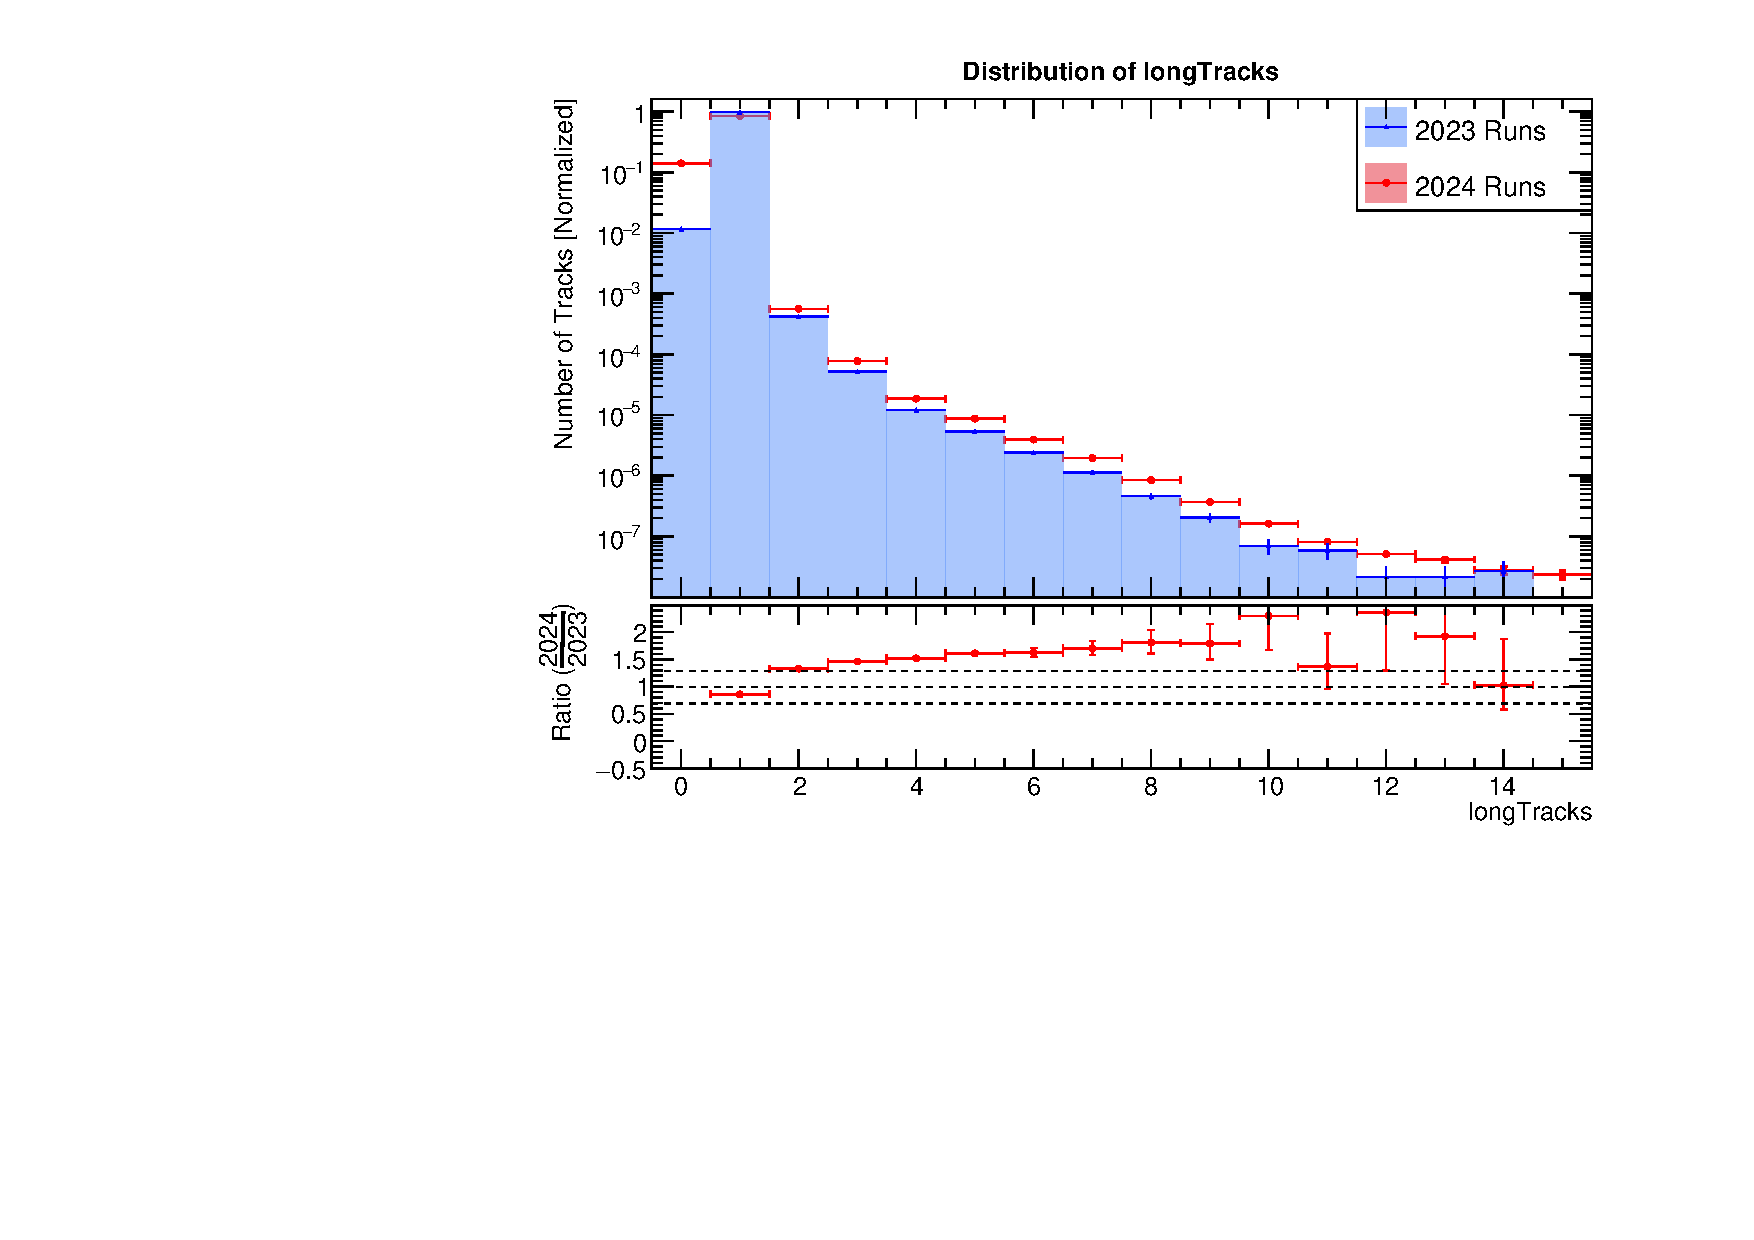
\includegraphics[width=\linewidth] {\plots/longTracks.pdf}
                \caption{Distribution of Number of Tracks}
            \end{figure}
        \end{column}
    \end{columns}
\end{frame}

\begin{frame}{Distribution of Track Charge}
    \begin{columns}
        \begin{column}{0.45\textwidth}
            \begin{itemize}
                \item We have a higher percentage of anti-muons
                \item Consistent with earlier observation of ``Much larger population of very high energy positive muons''  \href{https://indico.cern.ch/event/1407468/contributions/5915392/attachments/2851428/4985973/2024_conversions.pdf}{[see Talk]}    
            \end{itemize}
        \end{column}
        \begin{column}{0.8\textwidth}
            \begin{figure}
                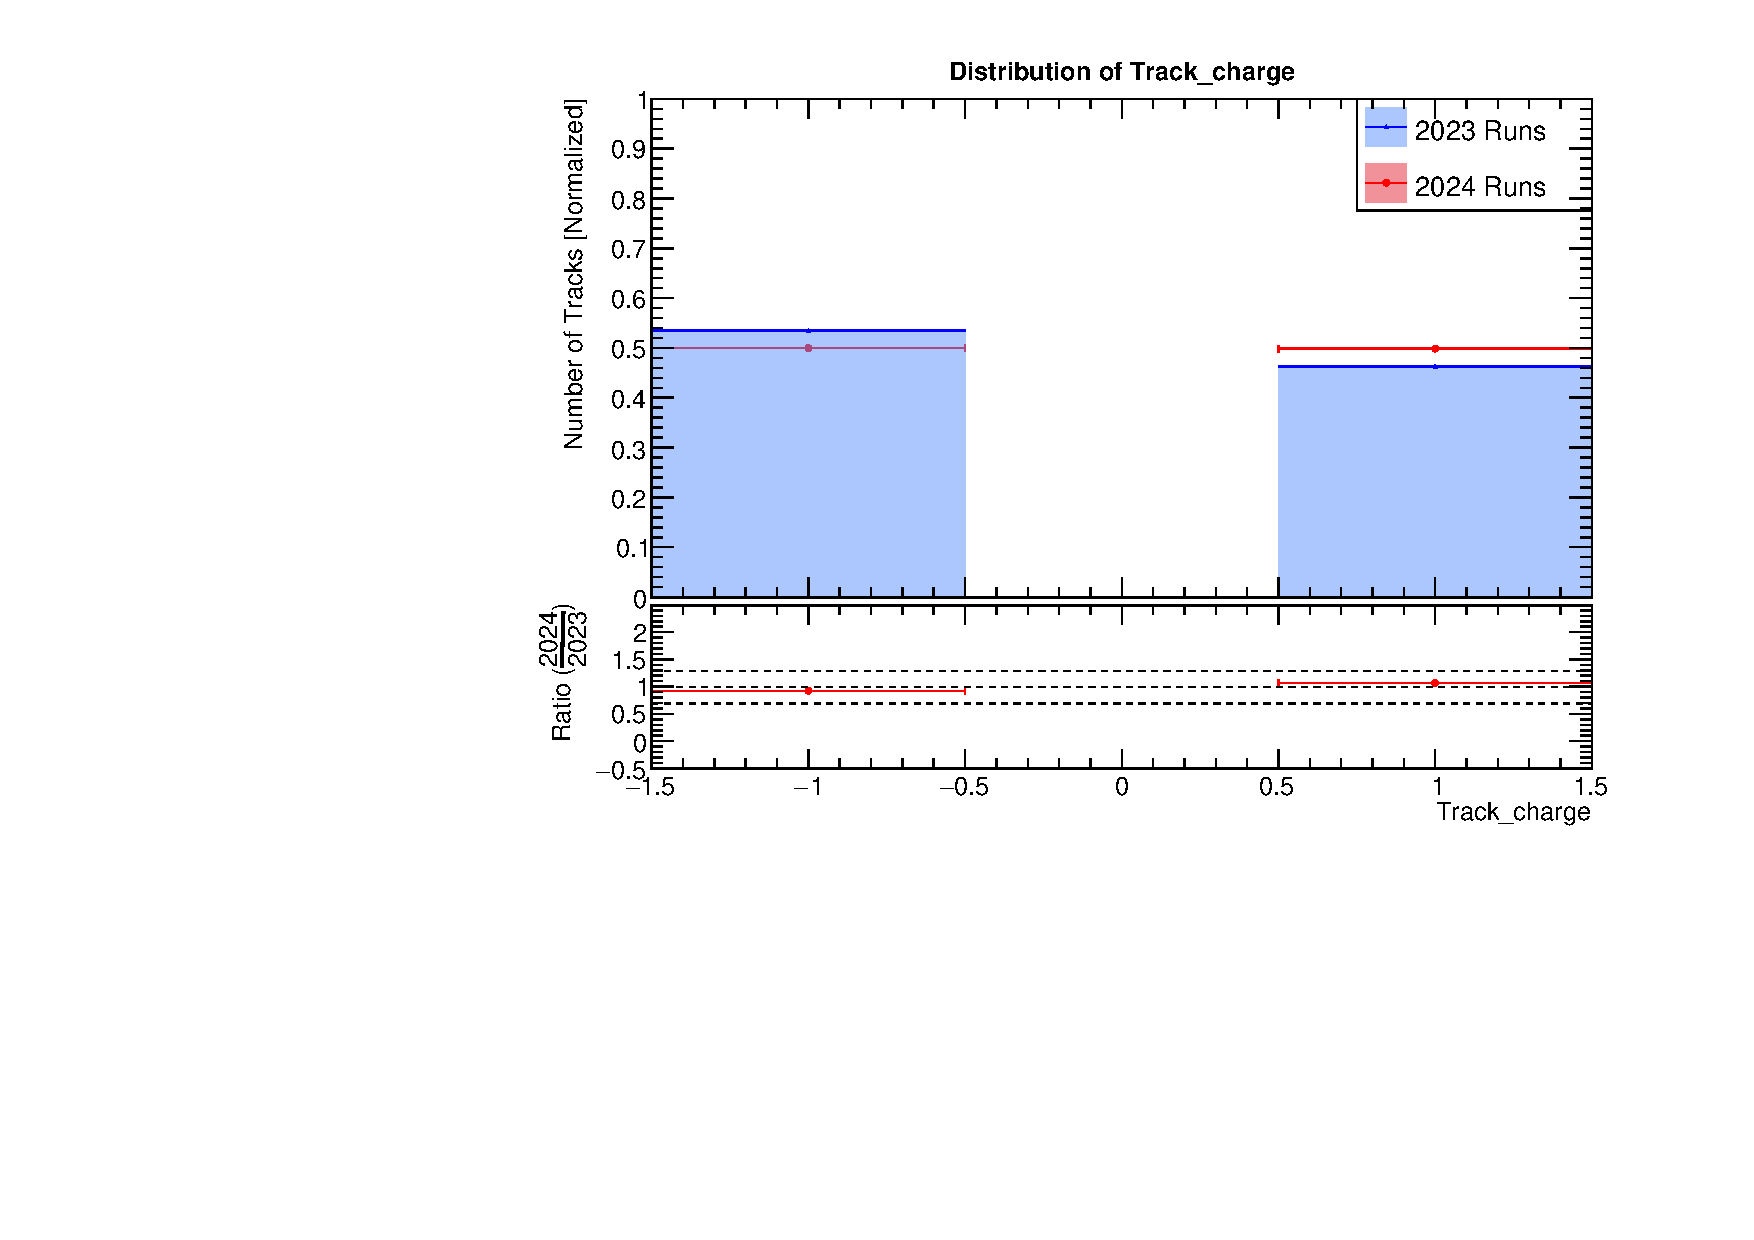
\includegraphics[width=\linewidth] {\plots/Track_charge.pdf}
                \caption{Distribution of Track Charge}
            \end{figure}
        \end{column}
    \end{columns}

\end{frame}

\begin{frame}{Distribution of Track $\chi^2$}
    \begin{columns}
        \begin{column}{0.45\textwidth}
            \begin{itemize}
                \item Overall we observe a lower Track $\chi^2$ in 2024
                \item Do we understand why?
            \end{itemize}
        \end{column}
        \begin{column}{0.8\textwidth}
            \begin{figure}
                % \begin{subfigure}
                \includegraphics[width=0.6\linewidth] {\plots/Track_chi2.pdf}
                \caption{Distribution of Track $\chi^2$}
                % \end{subfigure}
            \end{figure}
            \vspace{-0.7cm}
            \begin{figure}
                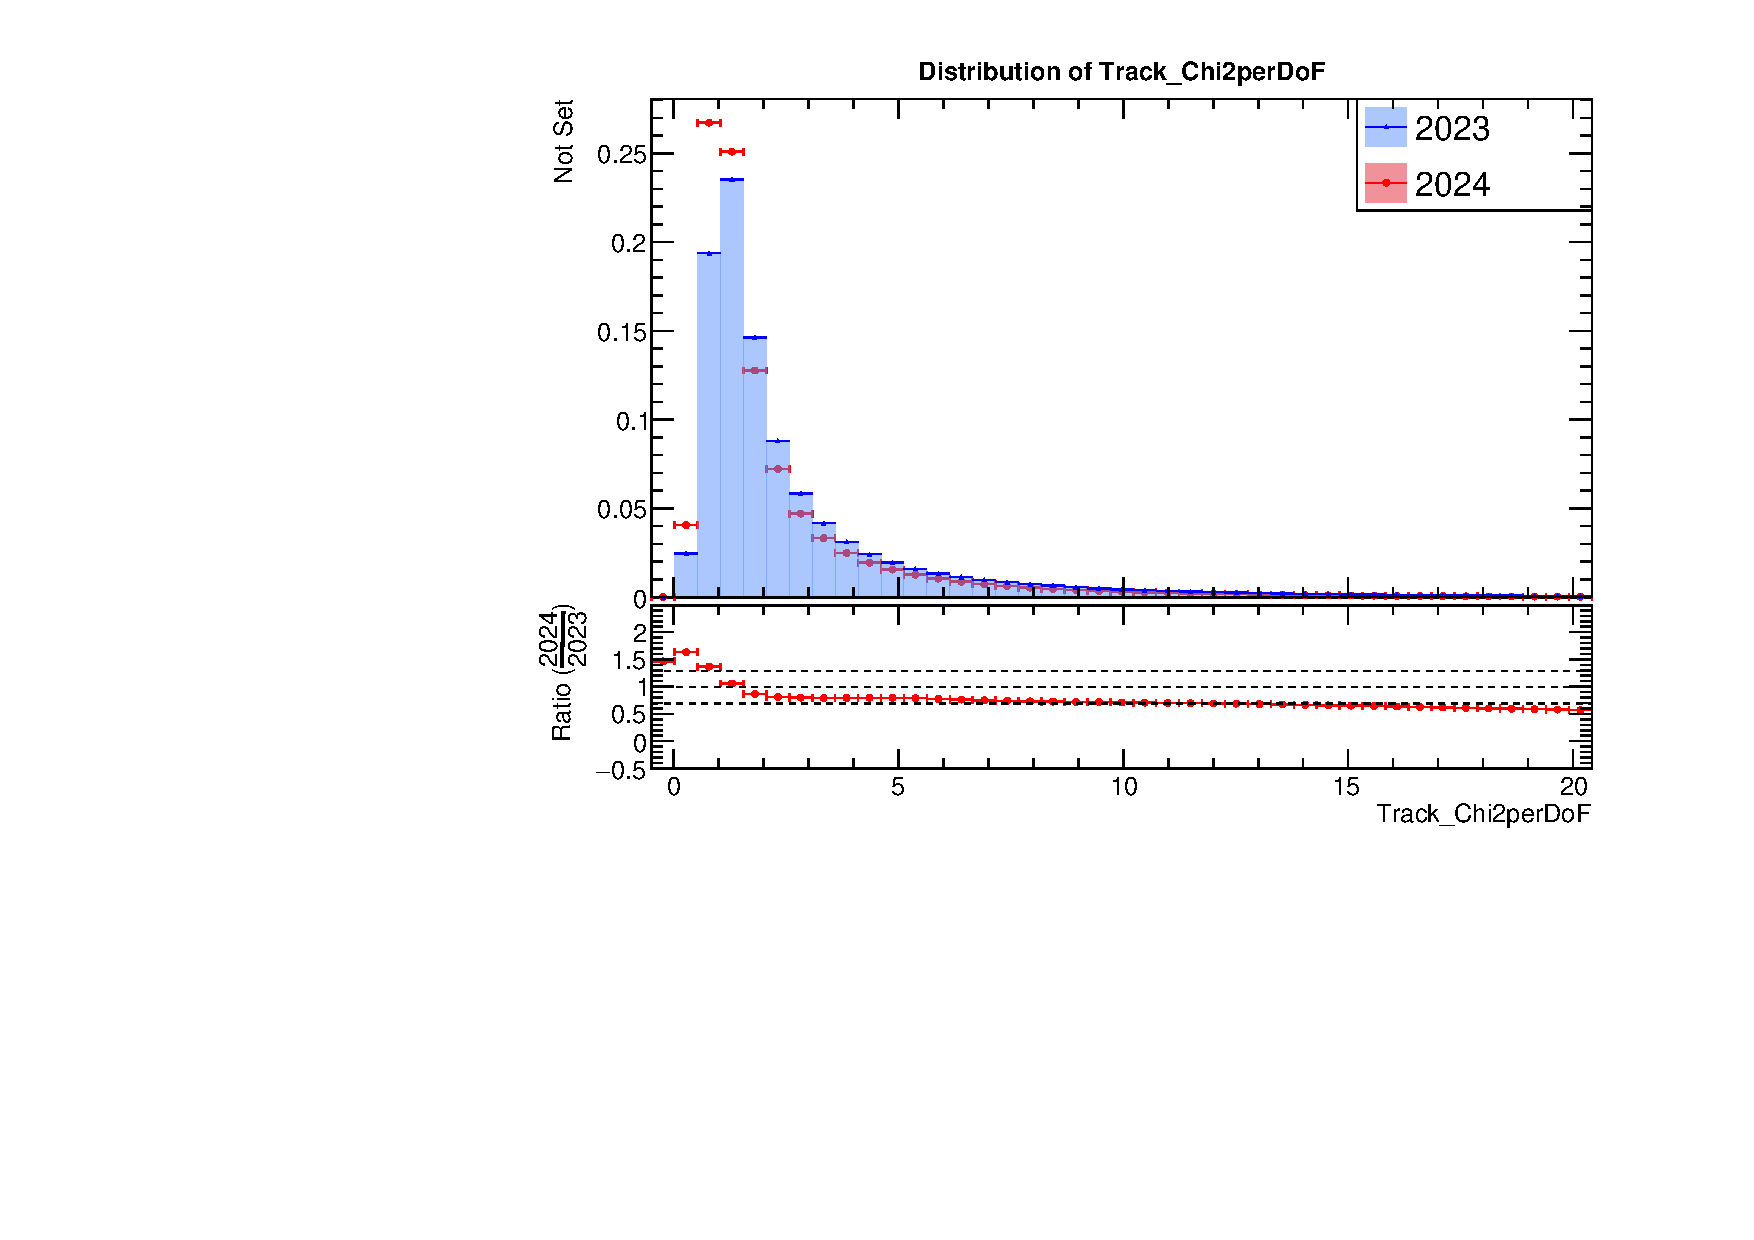
\includegraphics[width=0.6\linewidth] {\plots/Track_Chi2perDoF.pdf}
                \caption{Distribution of Track $\chi^2$ per DoF}
            \end{figure}
        \end{column}
    \end{columns}
\end{frame}

\begin{subframe}{Distribution of Track in Station [SKIP]}
    \begin{columns}
        \begin{column}{0.5\linewidth}
            \begin{tikzpicture}
                \draw (0,0) node[inner sep=0]{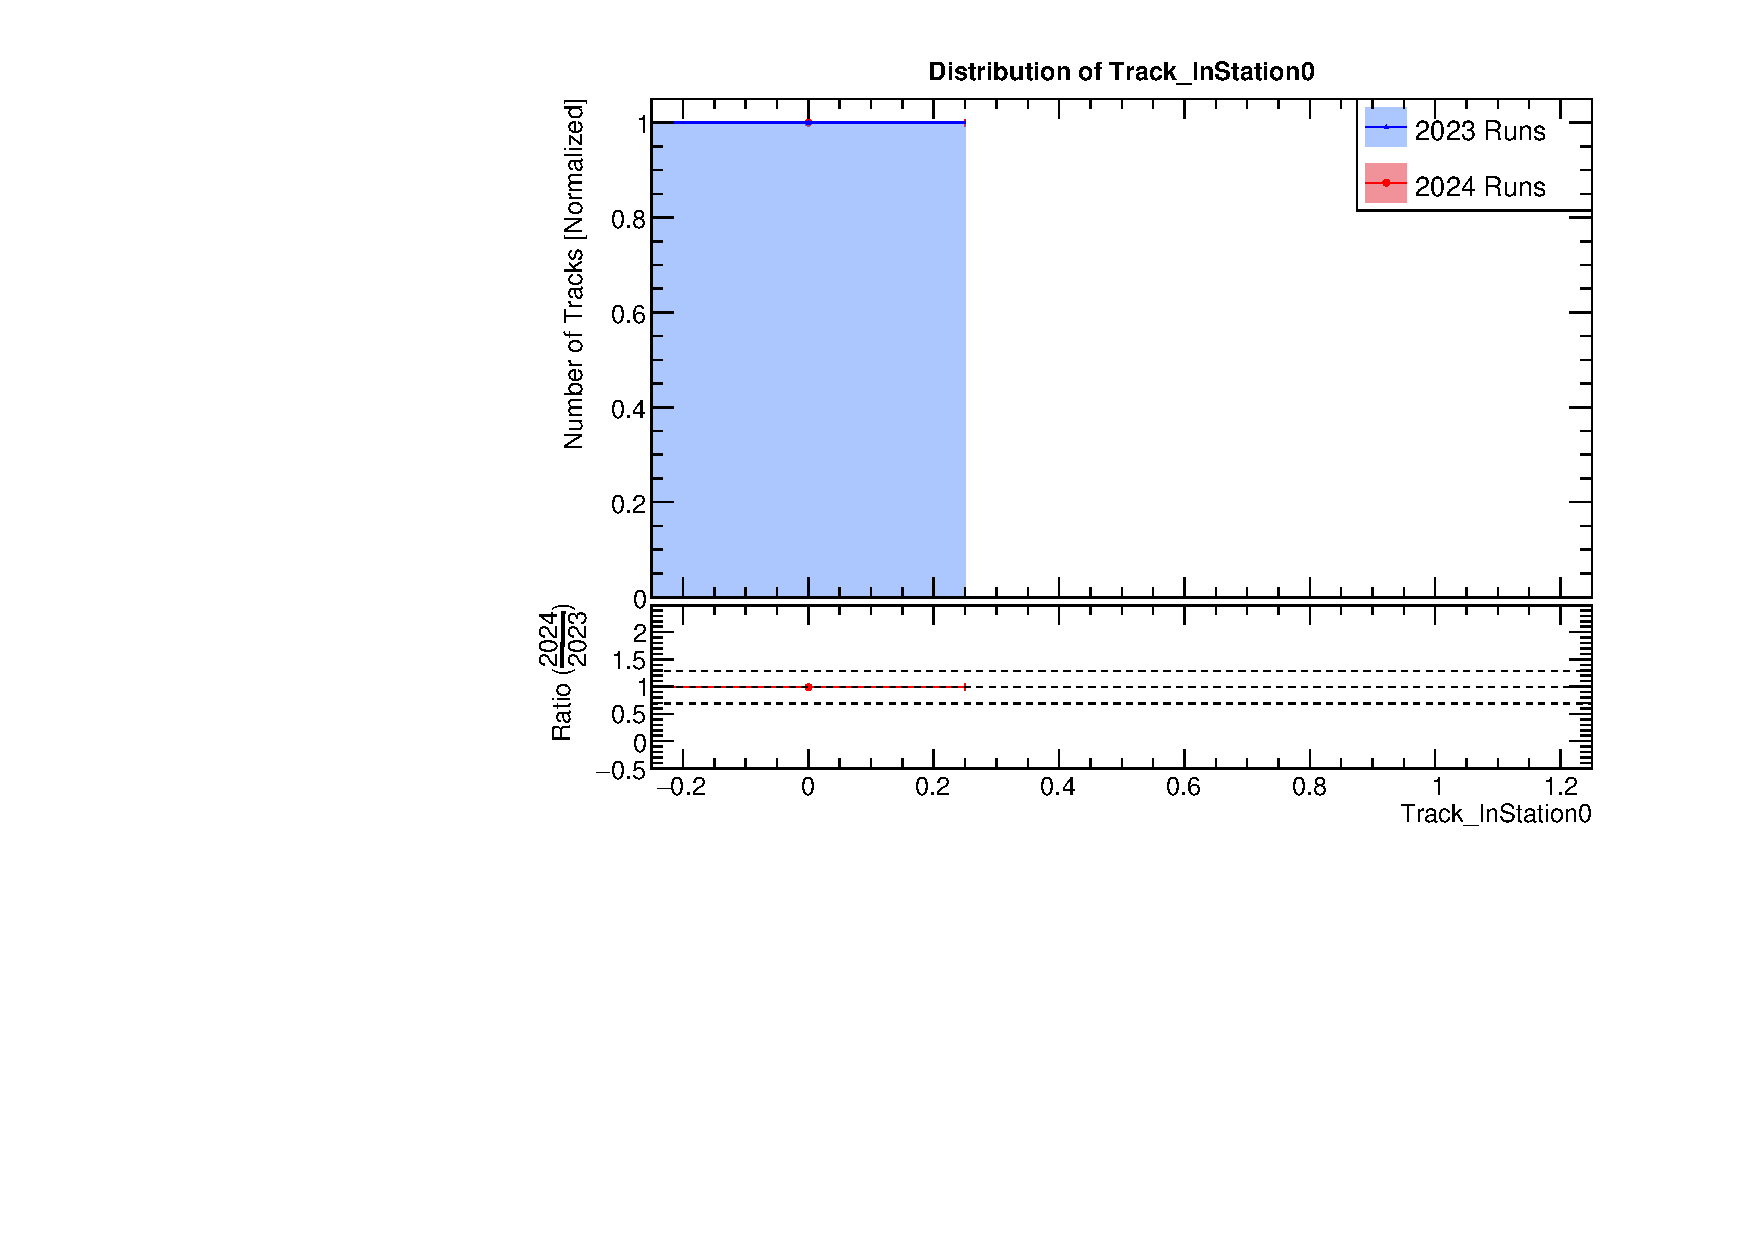
\includegraphics[width=\textwidth] {\plots/Track_InStation0.pdf}};
            \end{tikzpicture}
            \begin{tikzpicture}
                \draw (0,0) node[inner sep=0]{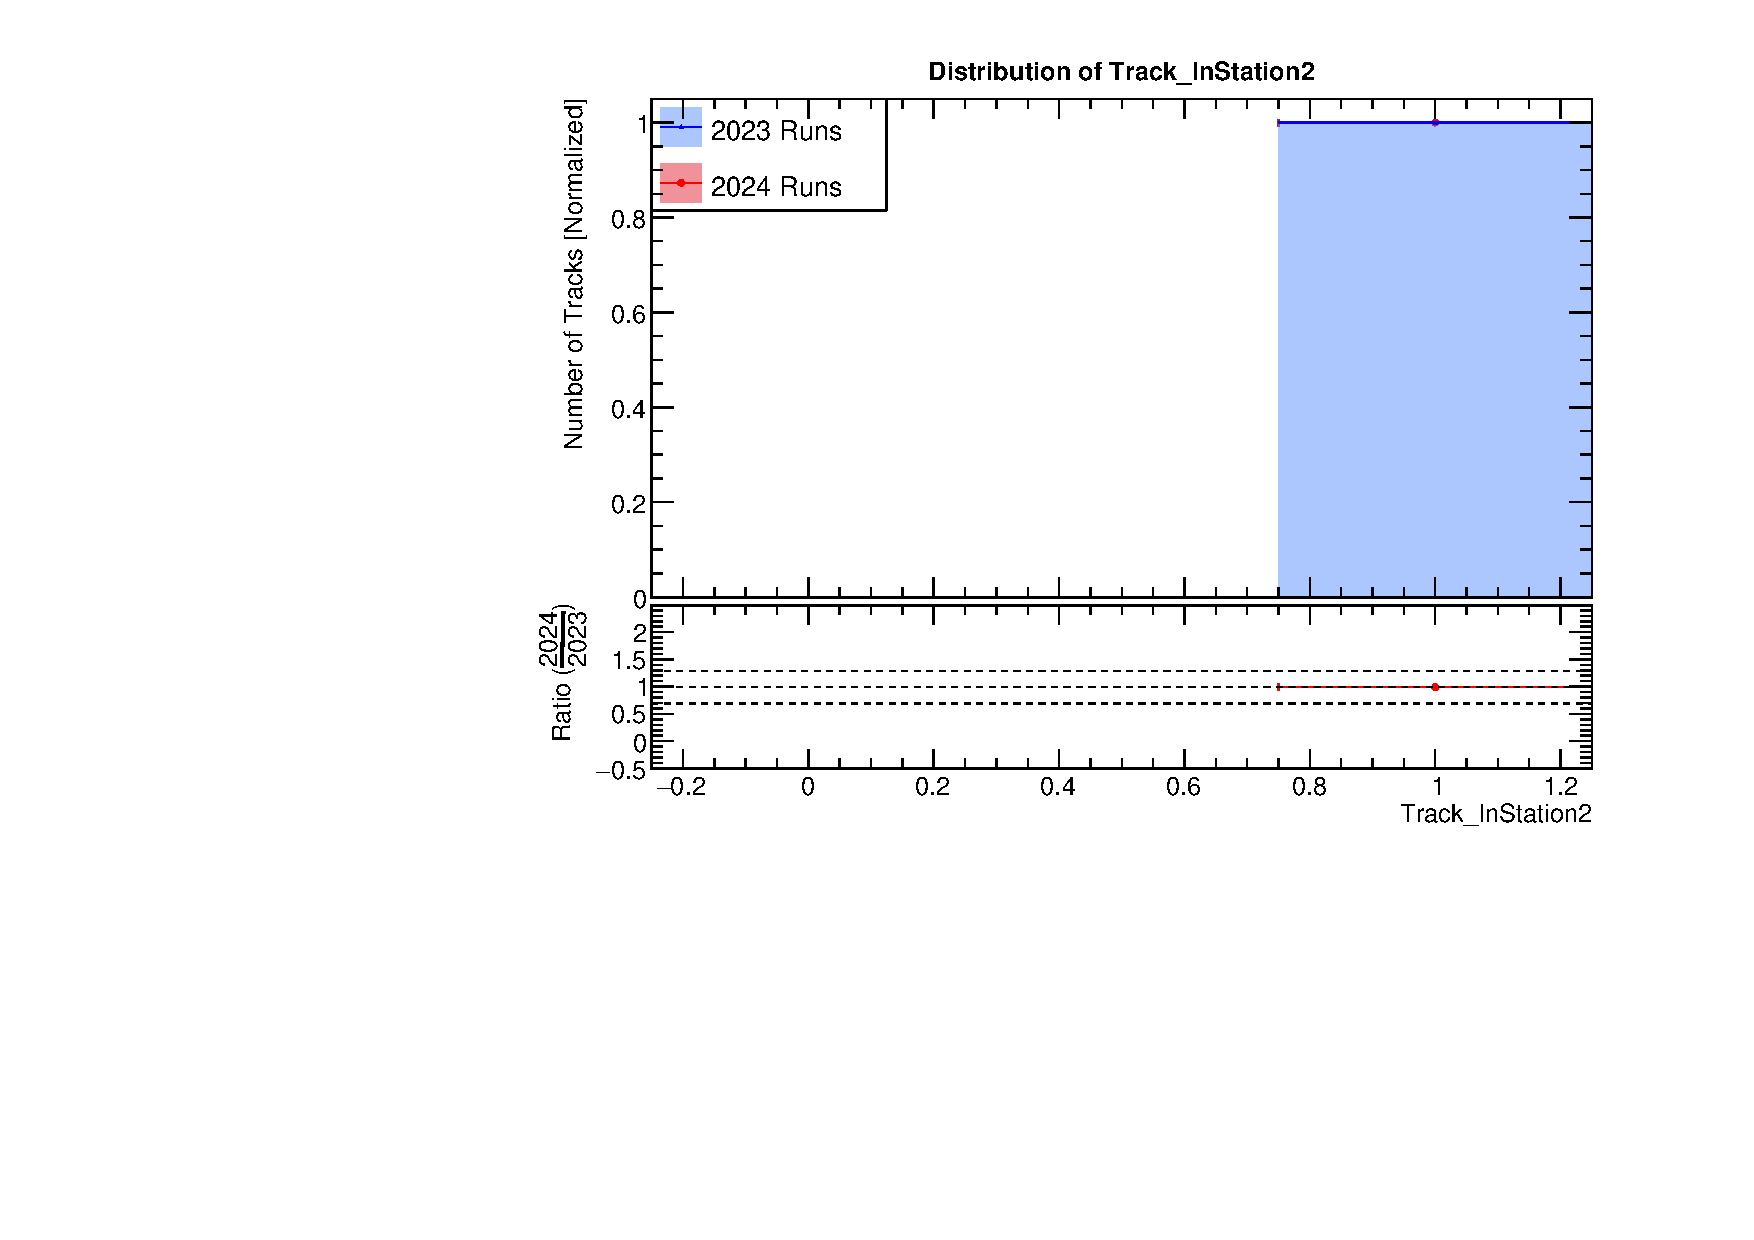
\includegraphics[width=\textwidth] {\plots/Track_InStation2.pdf}};
            \end{tikzpicture}
        \end{column}
        \begin{column}{0.5\linewidth}
            \begin{tikzpicture}
                \draw (0,0) node[inner sep=0]{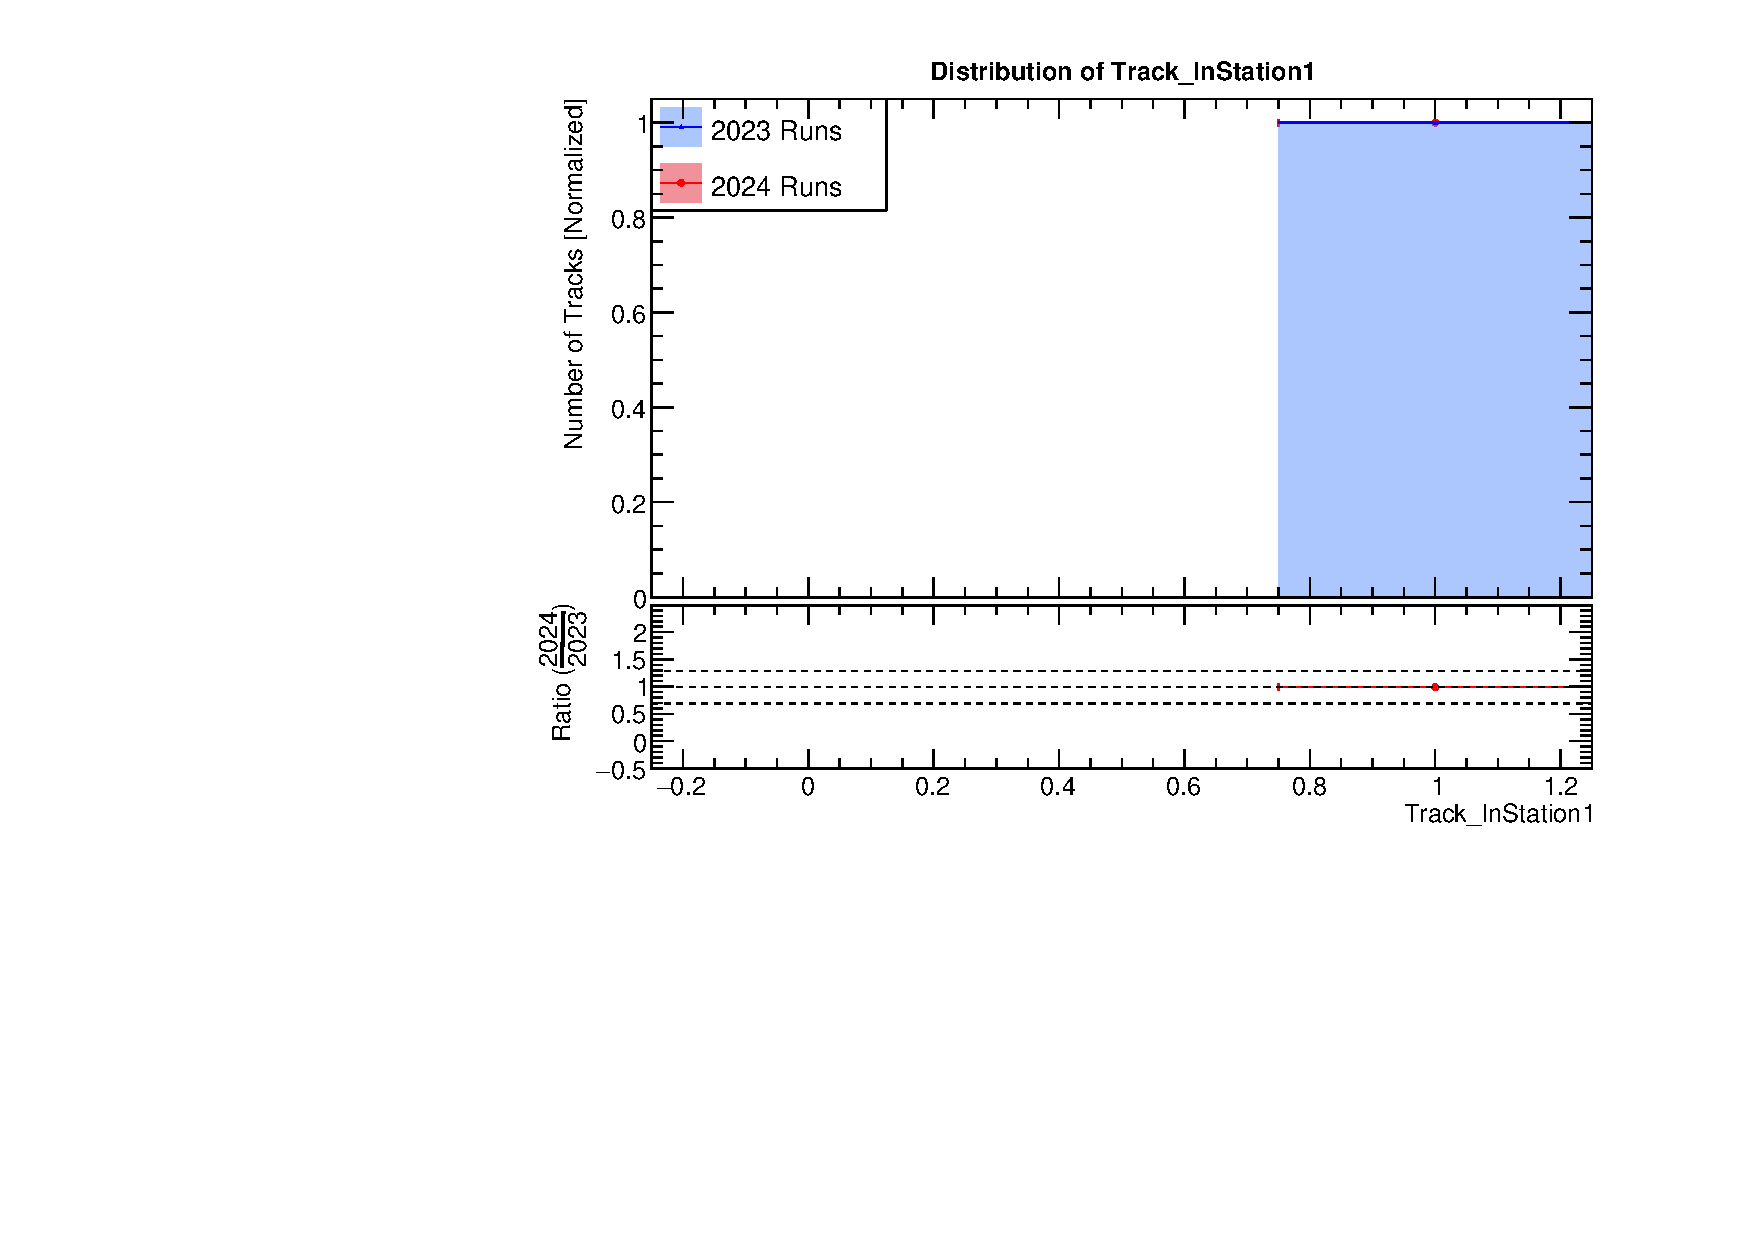
\includegraphics[width=\textwidth] {\plots/Track_InStation1.pdf}};
            \end{tikzpicture}
            \begin{tikzpicture}
                \draw (0,0) node[inner sep=0]{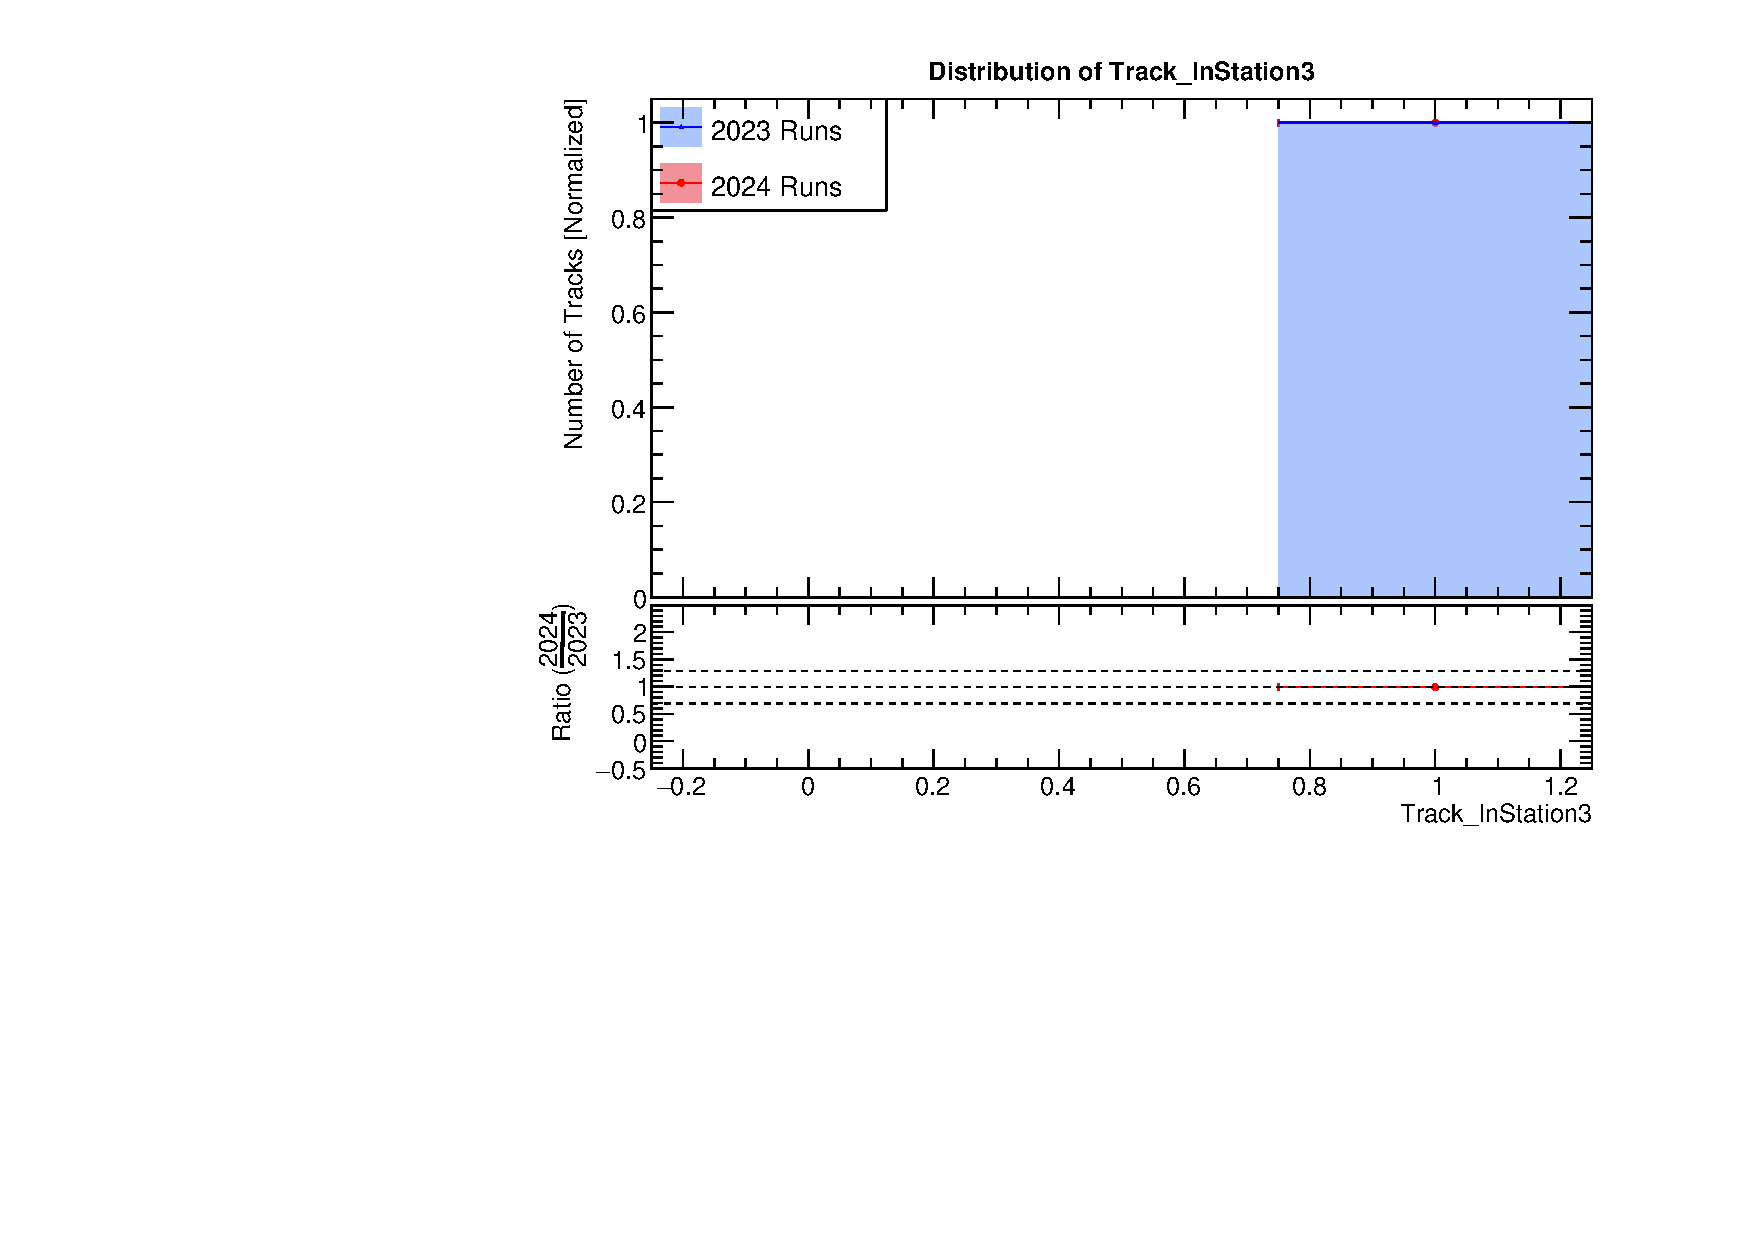
\includegraphics[width=\textwidth] {\plots/Track_InStation3.pdf}};
            \end{tikzpicture}
        \end{column}
    \end{columns}
    \scriptsize{There are always 0 tracks in Station0. Possibly an issue in NTupleDumper. Haven't located this yet.}
\end{subframe}

\begin{subframe}{Track\_nLayers [SKIP]}
    \begin{figure}
        \begin{tikzpicture}
            \draw (0,0) node[inner sep=0]{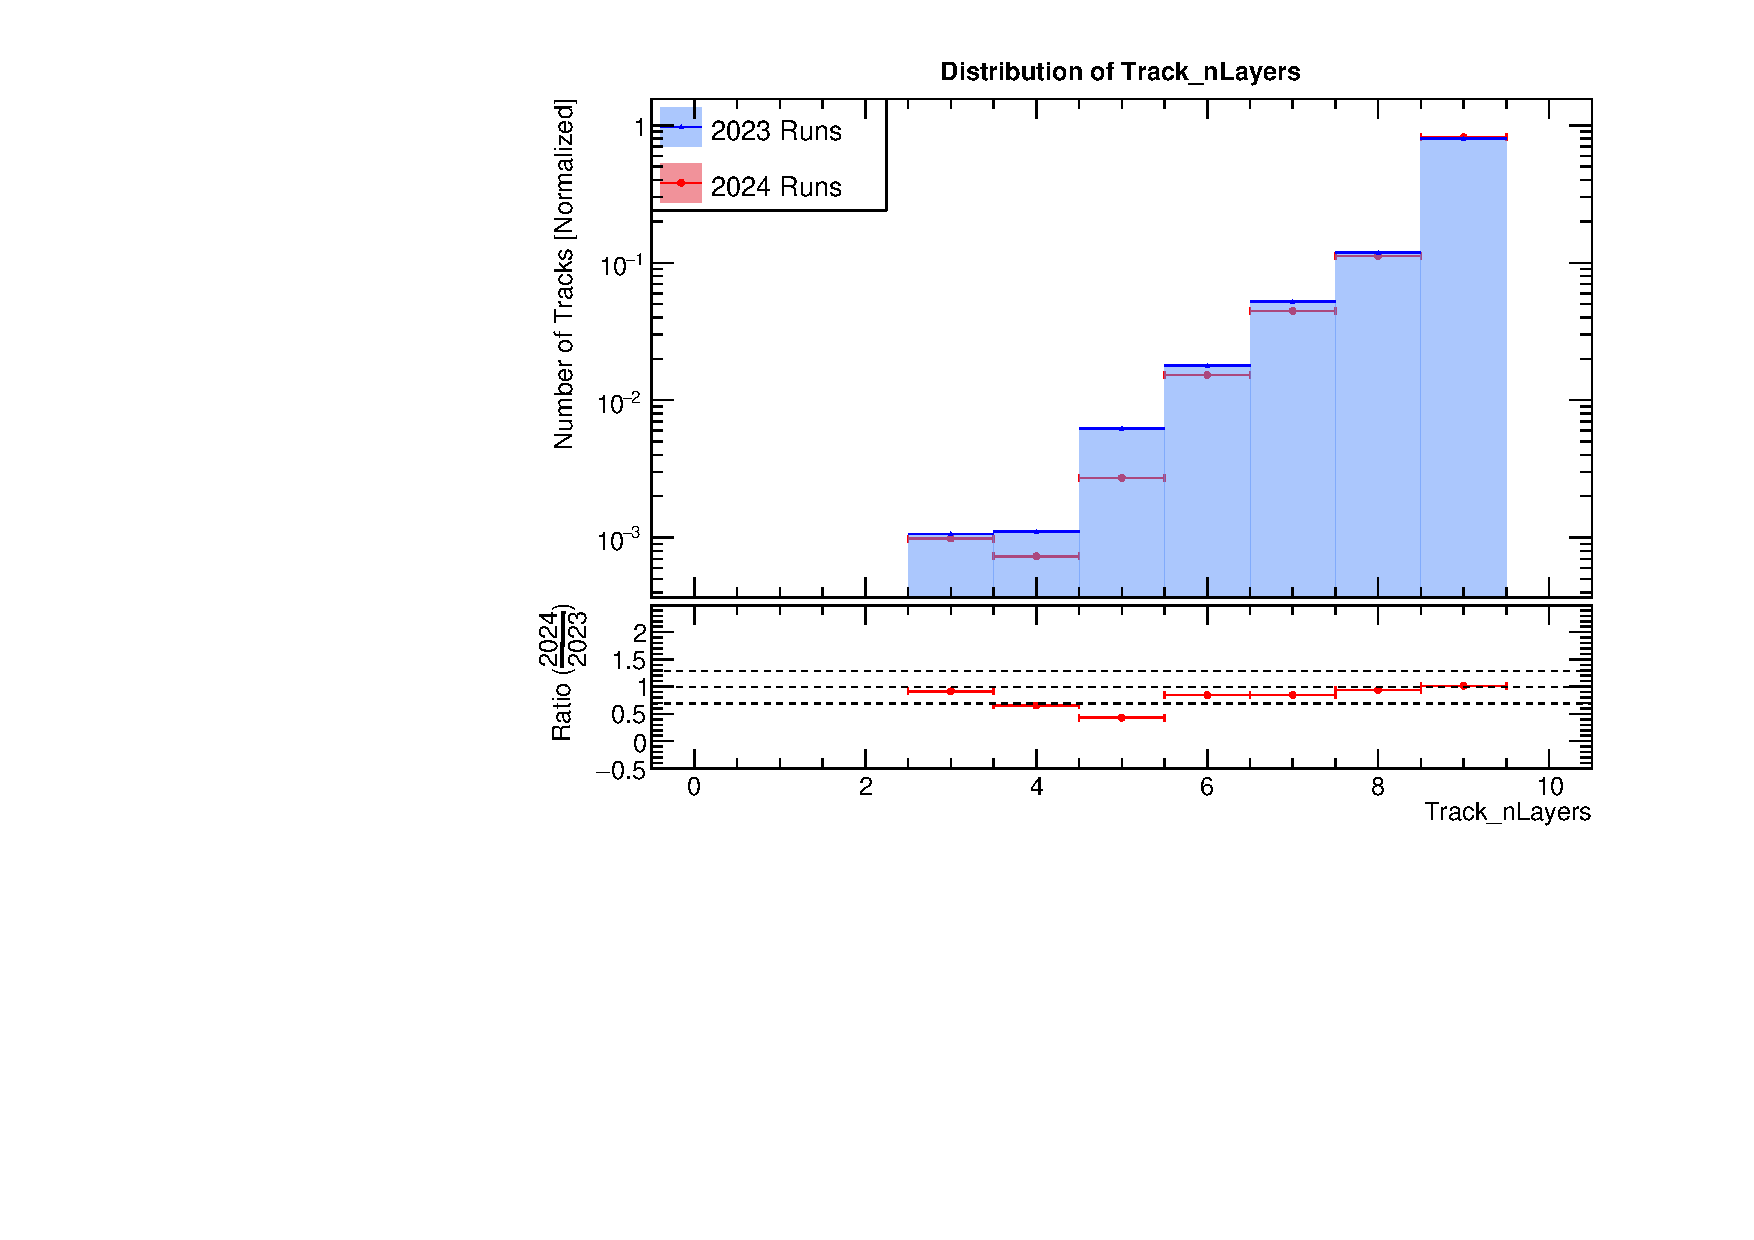
\includegraphics[width=\textwidth] {\plots/Track_nLayers.pdf}};
        \end{tikzpicture}
        \caption{Distribution of Track\_nLayers}
    \end{figure}
\end{subframe}

\begin{frame}{Track Propagation Error [SKIP]}
    \begin{figure}
        \begin{tikzpicture}
            \draw (0,0) node[inner sep=0]{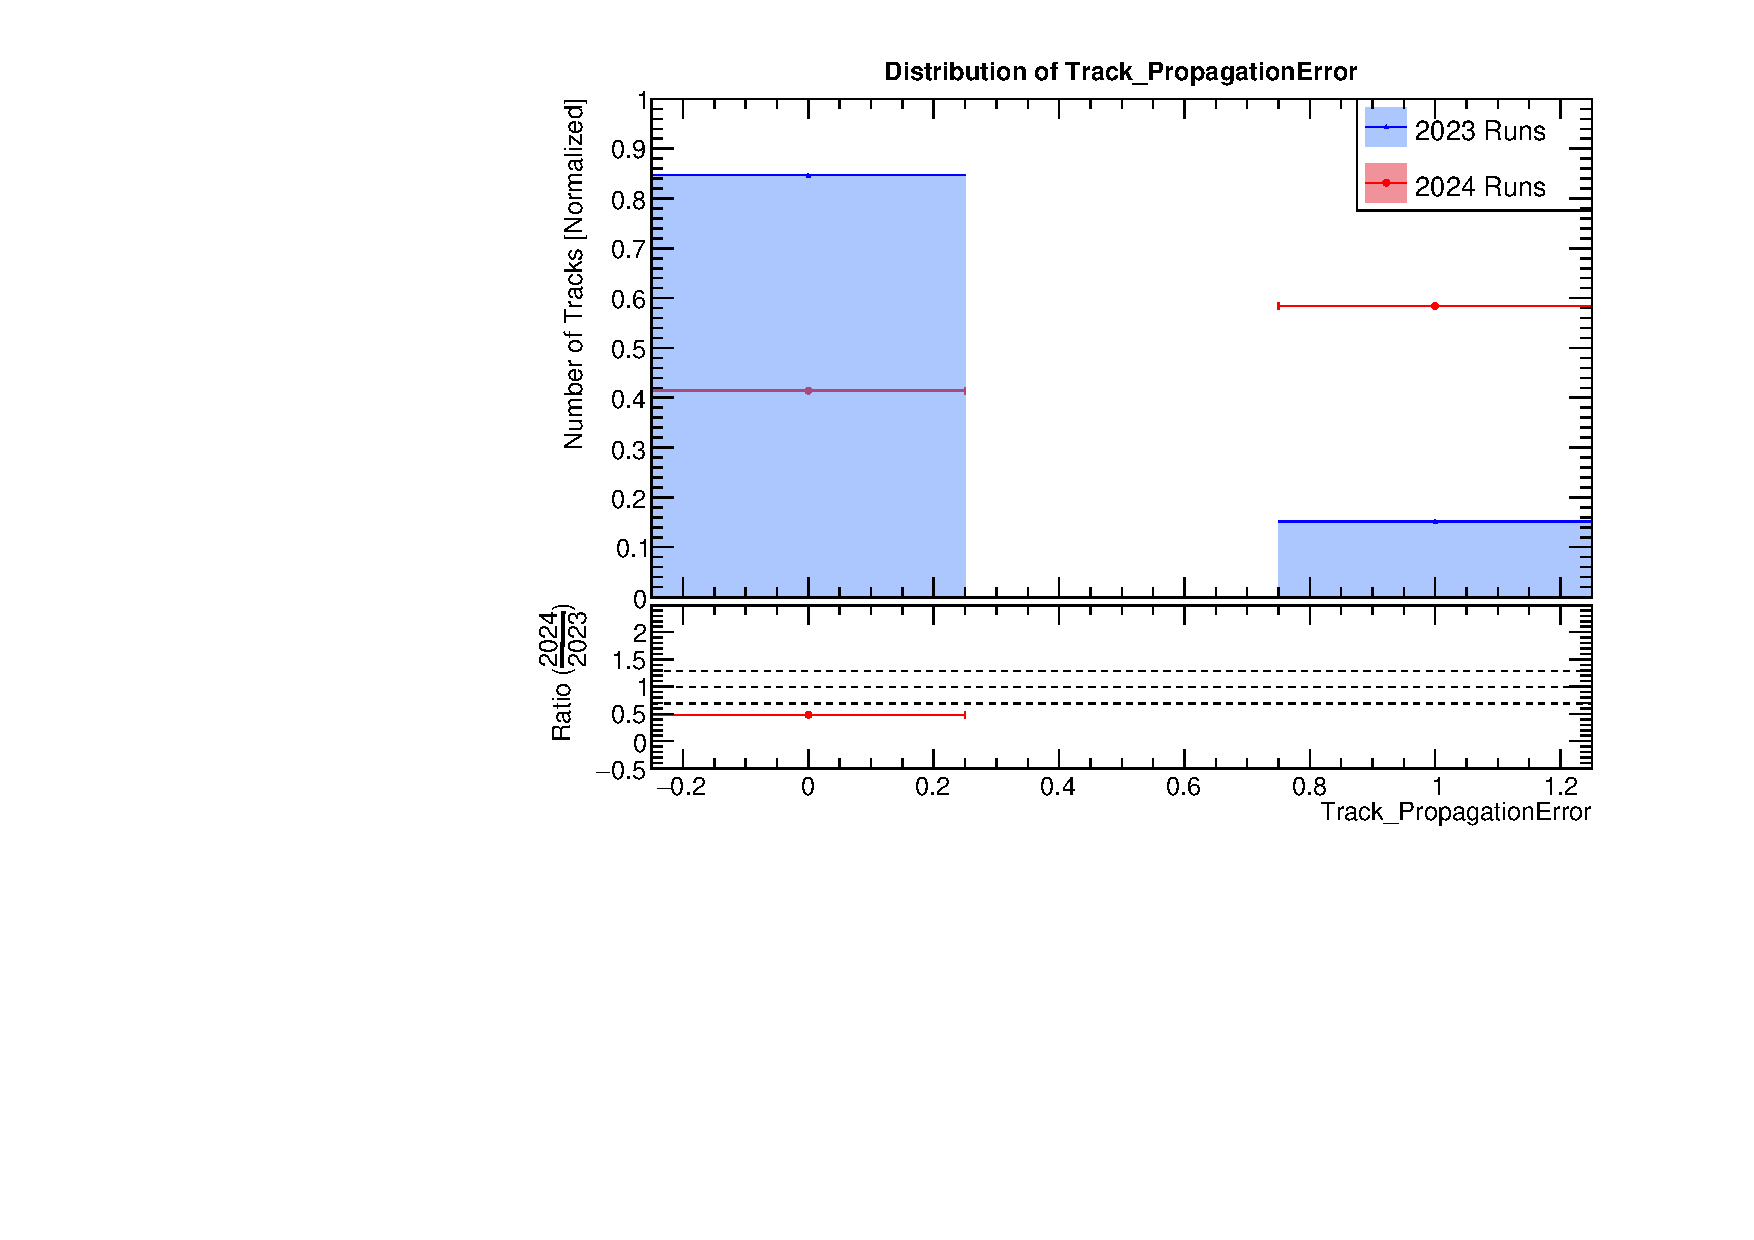
\includegraphics[width=\textwidth] {\plots/Track_PropagationError.pdf}};
        \end{tikzpicture}
        \caption{Distribution of Track Propagation Error}
    \end{figure}
\end{frame}